\Chapter{Módosító algoritmusok}

\Section{Az eloszlások távolságának mérése}

Az eloszlások ill. gyakoriságok távolságát több módon is mérhetjük.
Mivel nem cél a különböző metrikákkal kapott hibaértékek összehasonlítása, ezért lényegtelen hogy a mért és elvárt gyakoriságok vagy/és valószínűségek távolságát vizsgáljuk.
Ennek a hibának a mérésére a mért és elvárt értékek különbségéből kapható vektor normáival is megtörténhet:
\[
\vec{v} = \vec{e} - \vec{m},
\]
ahol az $\vec{e}$ az elvárt (\textit{expected}) és az $\vec{m}$ a mért (\textit{measured}) értékeket tartalmazza.

Az így kapott vektor 1-es normája által meghatározott érték megfelel a mért és elvárt adatok közötti abszolút különbségek összegével.
\[
\left\lVert\vec{v}\right\rVert_1 = \sum\limits_{i=1}^{n} |v_i|
\]
A 2--es norma a távolságok négyzetösszegének a gyökét adja vissza.
\[
\left\lVert\vec{v}\right\rVert_2 = \sqrt{\sum\limits_{i=1}^{n} |v_i|^2}
\]
A végtelen norma pedig a legnagyobb távolság abszolút értékét határozza meg.
\[
\left\lVert\vec{v}\right\rVert_\infty = \max\limits_{i=1}^{n} |v_i|
\]

Lehetséges ezeken kívül az átlagos négyzetes hibának (\textit{mean squared error, MSE}) számítása, amely nem sokban tér el a 2-es norma számításától.
\[
MSE(\vec{v}) = \frac{1}{n} \sum_{i=1}^{n}(v_i)^2
\]

Az eloszlások távolságának a mérésére a $\chi^2$-et szokták még alkalmazni, amellyel később meg lehet vizsgálni hogy milyen szignifikancia szinten egyezik meg az elvárt és mért értéksorozat.
\[
\chi^2=\sum_{i=1}^{n} \frac{(e_i - m_i)^2}{e_i}
\]

A fent említett metrikák közül az MSE-t valamint a $\chi^2$-et fogjuk alkalmazni.
Azért erre a kettőre esett a választás, mert az átlagos négyzetes hiba könnyen számolható négyzetes érték, valamint a $\chi^2$ számítása előnyös az illeszkedés vizsgálatra. 
Azért fontos hogy legyen egy négyzetes hiba számítás, mert az jobban kiemeli a távolságok közötti különbséget.

A $\chi^2$ számításánál minden különbségnégyzet a hozzá tartozó elvárt értékkel osztunk el, ezért nagyobb szórást enged meg ott, ahol magasabb az elvárt érték.
Ezzel szemben az MSE a különbségnégyzetek átlagát nézi, és nem enged meg sehol sem nagyobb szórást.
Emiatt a testek optimalizálásánál az utóbbi értéket fogjuk minimalizálni, és a $\chi^2$-et csak az ellenőrzésnél fogjuk használni.

\Section{Egyetlen pont mozgatása}
\label{sect:randmodification}

Ez a módszer a testet úgy módosítja, hogy mindig egy véletlenszerűen választott csúcspontját egy egység hosszúságú vektorral odébb helyezi.
A vektort a \ref{subs:randompoint} szakaszban említett módszerrel generáljuk.
Amennyiben a módosított test dobássorozata alapján kapott gyakoriságok jobbak mint az eredeti testé, az új testen végezzük el ugyan ezt a lépést, egyébként a módosítatlan testen.

%graph update!
\begin{figure}[h!]
	\centering
	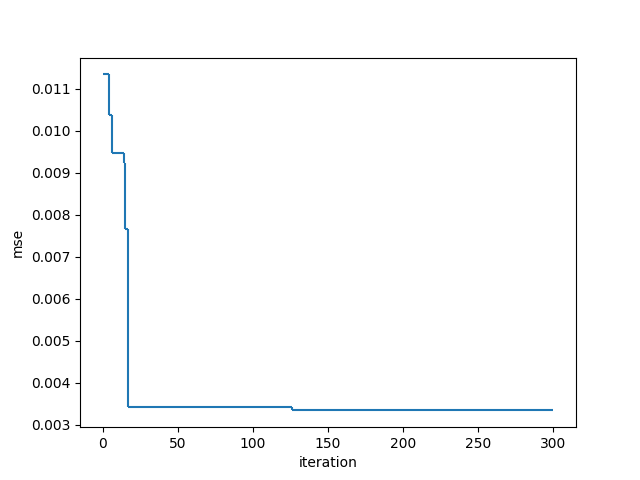
\includegraphics[scale=0.7]{images/randmodify_mse.png}
	\caption{Egyetlen pont elmozdításával kapott test módosítása közben mért legjobb MSE értékek.}
	\label{fig:randmodify_mse}
\end{figure}
A \ref{fig:randmodify_mse} grafikon egy tetraéder módosítása közben mért átlagos négyzetes hiba értékeket mutatja.
Az elvárt eloszlás [0.1, 0.2, 0.3, 0.4], leállás feltételéhez az iterációk száma $300$, a dobás sorozatok mérete pedig $N=200$.
A végén kapott testet 1000 dobára nézve $p=1.69920644248844\cdot10^{-77}$ szignifikancia szinten fogadjuk el.
Ebből arra tudunk következtetni, hogy a rossz módosítást a kis méretű dobássorozaton pontatlanul mért értékek miatt helyes módosításként kezelte.
Az így elmenett hibás állapotokból gyakran nem tudja az eljárás korrigálni jó irányba a testet.

Ez a módszer a véletlenszerű módosítások miatt nem tud konzisztensen egy megadott hibaküszöbhöz konvergálni, ezért futási paraméternek a módosító iterációk számát kell megadni hibaérték helyett.
Ez abból következik, hogy nem veszi figyelembe az elkövetett hibás módosításokat és nem von le következtetéseket a mért gyakoriságokból.

Mivel fix hosszúságú vektorral módosítjuk a testet és sosem lépünk vissza rosszabb hibaértéket adó testhez, így előfordulgat, hogy nem tudunk egy bizonyos hibaérték alá menni az optimalizálás során, mert a pontok egységsugarú környezetében található az optimális pozíciója.
Ezt úgy tudjuk kijavítani, hogy az iterációszám és a hibaértéktől függően csökkentjük a módosító vektorok hosszát.

A fent említett okok miatt érdemesebb más heurisztikával optimalizálni a testeket.

\Section{Oldallapok méretének módosítása}
\label{sect:facemodification}

Ez az algoritmus a csúcspontokat aszerint mozgatja, hogy oldallapokra nézve az elvárt és mért valószínűség hogyan viszonyul egymáshoz.
Ha az adott oldallap előfordulásán növelni szeretnénk akkor a csúcsokat lap súlypontjából kifelé mutató egység hosszúságú vektorokkal mozdítjuk el, egyébként a csúcsokat a súlypont felé mozgatjuk.
A \ref{fig:facemodification} ábrán látható kék vektorok felelnek az oldallap növeléséért, a vörösek pedig annak csökkentéséért.

\begin{figure}[h!]
	\centering
	\begin{tikzpicture}
		\node [label={[shift={(-0.2,-0.1)}]$C$},inner sep=0] (C) at (4,3) {};
		\node [label={[shift={(-0.2,0)}]$P_1$},inner sep=0] (P1) at (0,0) {};
		\node [label={[shift={(0.3,-0.2)}]$P_2$},inner sep=0] (P2) at (5,7) {};
		\node [label={[shift={(0.2,0)}]$P_3$},inner sep=0](P3) at (7,2) {};
		\draw (P1) -- (P2) -- (P3) -- (P1);
		\draw [dashed] (C) -- (P1);
		\draw [dashed] (C) -- (P2);
		\draw [dashed] (C) -- (P3);
		\node [inner sep=0] (out1) at (-0.8,-0.6) {};
		\node [inner sep=0] (out2) at (5.24,7.97) {};
		\node [inner sep=0] (out3) at (7.95,1.68) {};
		\draw [->, draw=blue] (P1) -- (out1);
		\draw [->, draw=blue] (P2) -- (out2);
		\draw [->, draw=blue] (P3) -- (out3);
		\draw [dotted] (out1) -- (out2) -- (out3) -- (out1);
		\node [inner sep=0] (in1) at (0.8,0.6) {};
		\node [inner sep=0] (in2) at (4.76,6.03) {};
		\node [inner sep=0] (in3) at (6.05,2.32) {};
		\draw [->, draw=red] (P1) -- (in1);
		\draw [->, draw=red] (P2) -- (in2);
		\draw [->, draw=red] (P3) -- (in3);
		\draw [dotted] (in1) -- (in2) -- (in3) -- (in1);
	\end{tikzpicture}
	\caption{Oldallap méretének változtatása egység hosszúságú vektorral.}
	\label{fig:facemodification}
\end{figure}
\begin{figure}[h!]
	\centering
	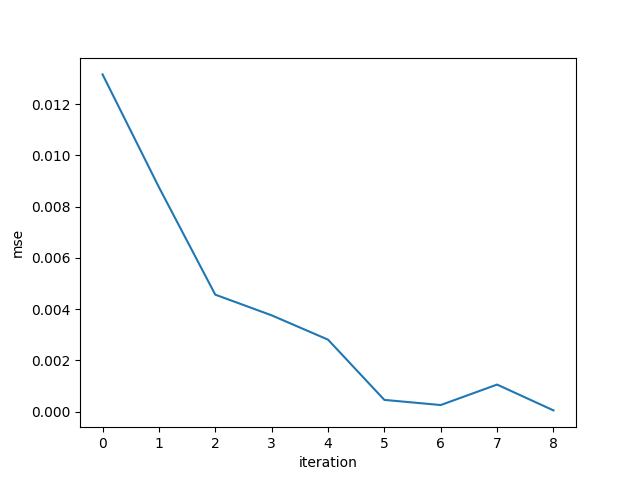
\includegraphics[scale=0.7]{images/facemodify_mse.png}
	\caption{Az oldallapok méretének módosításával mért MSE értékek az iterációk függvényében.}
	\label{fig:facemodify_mse}
\end{figure}

A \ref{fig:facemodify_mse} grafikonon látható egy tetraéder módosítása közben kapott átlagos négyzetes hibák.
A várt eloszlás [0.1, 0.2, 0.3, 0.4], a dobássorozatok mérete $N=1000$, a hibaküszöb pedig $0.00001$.
A végén kapott testet $1000$ dobásra nézve $p=0.636748542457662$ megbízhatósági szinten lehet elfogadni.

A \ref{subs:randompoint} szakaszban bemutatott módszerhez képest látványosan gyorsabb, és egyértelműen konvergál az elvárt eloszláshoz.
Mivel az algoritmus az aktuálisan mért eloszlásokhoz képest módosítja a lapok méretét, így az esetlegesen elkövetett hibákat folyamatosan tudja javítani, valamint mivel sokkal gyorsabban konvergál, így nyugodtan adhatunk meg nagyobb dobásméretet, amellyel tovább tudjuk csökkenteni az esetleges fals méréseket.

\Section{Módosítás az arányok figyelembe vételével}

Ez a folyamat szinte teljes mértékben megegyezik az előző pontban leírt metódushoz.
Az egyetlen lényeges különbség annyi, hogy az oldallapokat a gyorsabb konvergencia miatt nem egység hosszú vektorokkal módosítjuk.
A módosító vektorok hossza függ az oldallapokhoz mért és elvárt valószínűségek különbségétől, hogy a nagyobb eltérések esetében drasztikusabban tudjuk az oldallapokat módosítani.
Olyan eset is előfordulhat, hogy az oldallap ideális méretének eléréséhez az oldallapot fél egység hossz vektorokkal kéne növelnünk, és ezt a méretet a \ref{sect:facemodification} szakaszban leírt függvénnyel nem tudjuk elérni.